\documentclass[]{article}

% Imported Packages
%------------------------------------------------------------------------------
\usepackage{amssymb}
\usepackage{amstext}
\usepackage{amsthm}
\usepackage{amsmath}
\usepackage{enumerate}
\usepackage{fancyhdr}
\usepackage[margin=1in]{geometry}
\usepackage{graphicx}
%\usepackage{extarrows}
%\usepackage{setspace}
%\usepackage{xcolor}
\usepackage{color}
\usepackage{float}
\usepackage{svg}
\usepackage{hyperref}
%------------------------------------------------------------------------------

% Header and Footer
%------------------------------------------------------------------------------
\pagestyle{plain}  
\renewcommand\headrulewidth{0.4pt}                                      
\renewcommand\footrulewidth{0.4pt}                                    
%------------------------------------------------------------------------------

% Title Details
%------------------------------------------------------------------------------
\title{Deliverable \#1: What’s That Dish Software Requirement Specification (SRS)}
\author{SE 3A04: Software Design II -- Large System Design}
\date{}
                            
%------------------------------------------------------------------------------

% Document
%------------------------------------------------------------------------------
\begin{document}

\maketitle	
\noindent{\bf Tutorial Number:} T03\\
{\bf Group Number:} G03 \\
{\bf Group Members:} 
\begin{itemize}
	\item Imran Chowdhury
	\item Michael Roberts
	\item Sathurshan Arulmohan
	\item Tanisha Tasnin
	\item Zifan Si
\end{itemize}

\newpage
\section{Introduction}
\label{sec:introduction}
% Begin Section

This document outlines What's That Dish, an Android mobile application for identifying food and dishes. The document will cover the application's purpose, overall product description, stakeholder use cases, main business events from perspective of various viewpoints, and product requirements.


\subsection{Purpose}
\label{sub:purpose}
% Begin SubSection
This document focuses on the functional and non-functional requirements of What's That Dish. The intended audience includes internal stakeholders such as the client, software developers, and software architects.
% End SubSection

\subsection{Scope}
\label{sub:scope}
% Begin SubSection
What’s That Dish, the intelligent food identification application, helps users identify dishes based on their input of an image, text description, or ingredients list submission. The system utilizes three expert modules, Image Recognition, Text Description, and Ingredient-Based Experts for identification. Additionally, the system provides nutritional information and restaurant recommendations while storing user data to deliver personalized food suggestions.

Users are required to create an account on What’s That Dish to access its features. “What’s that dish?!”, the app’s primary and default mode, allows users to submit dish details (photo, text, and/or ingredient list), and the system processes the input through the combined effort of the three expert modules. “Add Custom Recipe” and “Personalized Recommendations” serve as secondary features that expand the functionality of the platform. In “Add Custom Recipe,” the system prompts users to provide detailed recipes of their unique dishes including ingredients, portion sizes, and preparation steps. This feature contributes to the development of a diverse and comprehensive food database for the What’s That Dish community. Meanwhile, the “Personalized Recommendations” mode curates a tailored experience by suggesting dishes based on a user’s previous inquiries and preferences, while also recommending local restaurants based on location data.

What’s That Dish aims to be every foodie’s go-to solution when they stumble upon a dish on a social media applcation, in real life, or anywhere else that sparks their curiosity, yet they have no idea what it is or where it originates from. By offering multiple input options, the platform ensures flexibility and accessibility for a wide range of users. The application seeks to foster an interactive community where users contribute recipes, enriching the platform’s database and promoting food discovery. By cultivating a user-driven ecosystem, the application not only enhances personalized recommendations but also encourages cultural exchange through shared recipes. Additionally, the system aims to establish partnerships with local restaurants, increasing food exploration opportunities while supporting the restaurant industry.

% End SubSection

\subsection{Definitions, Acronyms, and Abbreviations}
\label{sub:definitions_acronyms_and_abbreviations}
% Begin SubSection
\begin{itemize}
	\item Provide the definitions of all terms, acronyms, and abbreviations required to properly interpret the SRS.
	\item This should be in alphabetical order.
\end{itemize}
% End SubSection

\subsection{References}
\label{sub:references}
% Begin SubSection
\bibliographystyle{IEEEtran}
\renewcommand{\refname}{}  % Remove "References" title
\vspace{-7mm}  % Adjust spacing before bibliography
\bibliography{references}
% End SubSection

\subsection{Overview}
\label{sub:overview}
% Begin SubSection
\begin{itemize}
	\item Describe what the remainder of the document/SRS contains.\\
	(e.g. "Section 2 discusses...Section 3...")
%	\item Explain how the SRS is organized
\end{itemize}
% End SubSection

% End Section

\section{Overall Product Description}
\label{sec:overall_description}

\subsection{Product Perspective}
\label{sub:product_perspective}

"What’s That Dish" is an Android-based mobile application for food identification, allowing users to recognize and learn about any dish they come across online, whether it's a screenshot from a social media applcation or a Facebook post. Similar to Google Lens, Yuka, and MyFitnessPal, it enables users to scan food items for nutritional information or perform image-based searches. However, "What’s That Dish?!" sets itself apart with a multi-modal identification approach, letting users identify dishes via photos, text descriptions, or ingredient lists, rather than relying solely on image recognition. The platform integrates Google Maps API to recommend nearby restaurants serving identified dishes, sharing similarities with applications like OpenTable and Zomato. Additionally, the application connects to external resources through third-party APIs, such as the Canada Nutrient File database for nutrition data aligned with Health Canada guidelines and machine learning models for image and natural language processing.

The application also includes two secondary features: Custom Recipe Submission, which allows users to add recipes by providing ingredients, portions, and preparation steps, and Personalized Recommendations, which uses machine learning to suggest dishes based on user preferences and search history. These features expand the food database with community-generated content while delivering a personalized and engaging food discovery experience.


\begin{figure}[H]
    \centering
    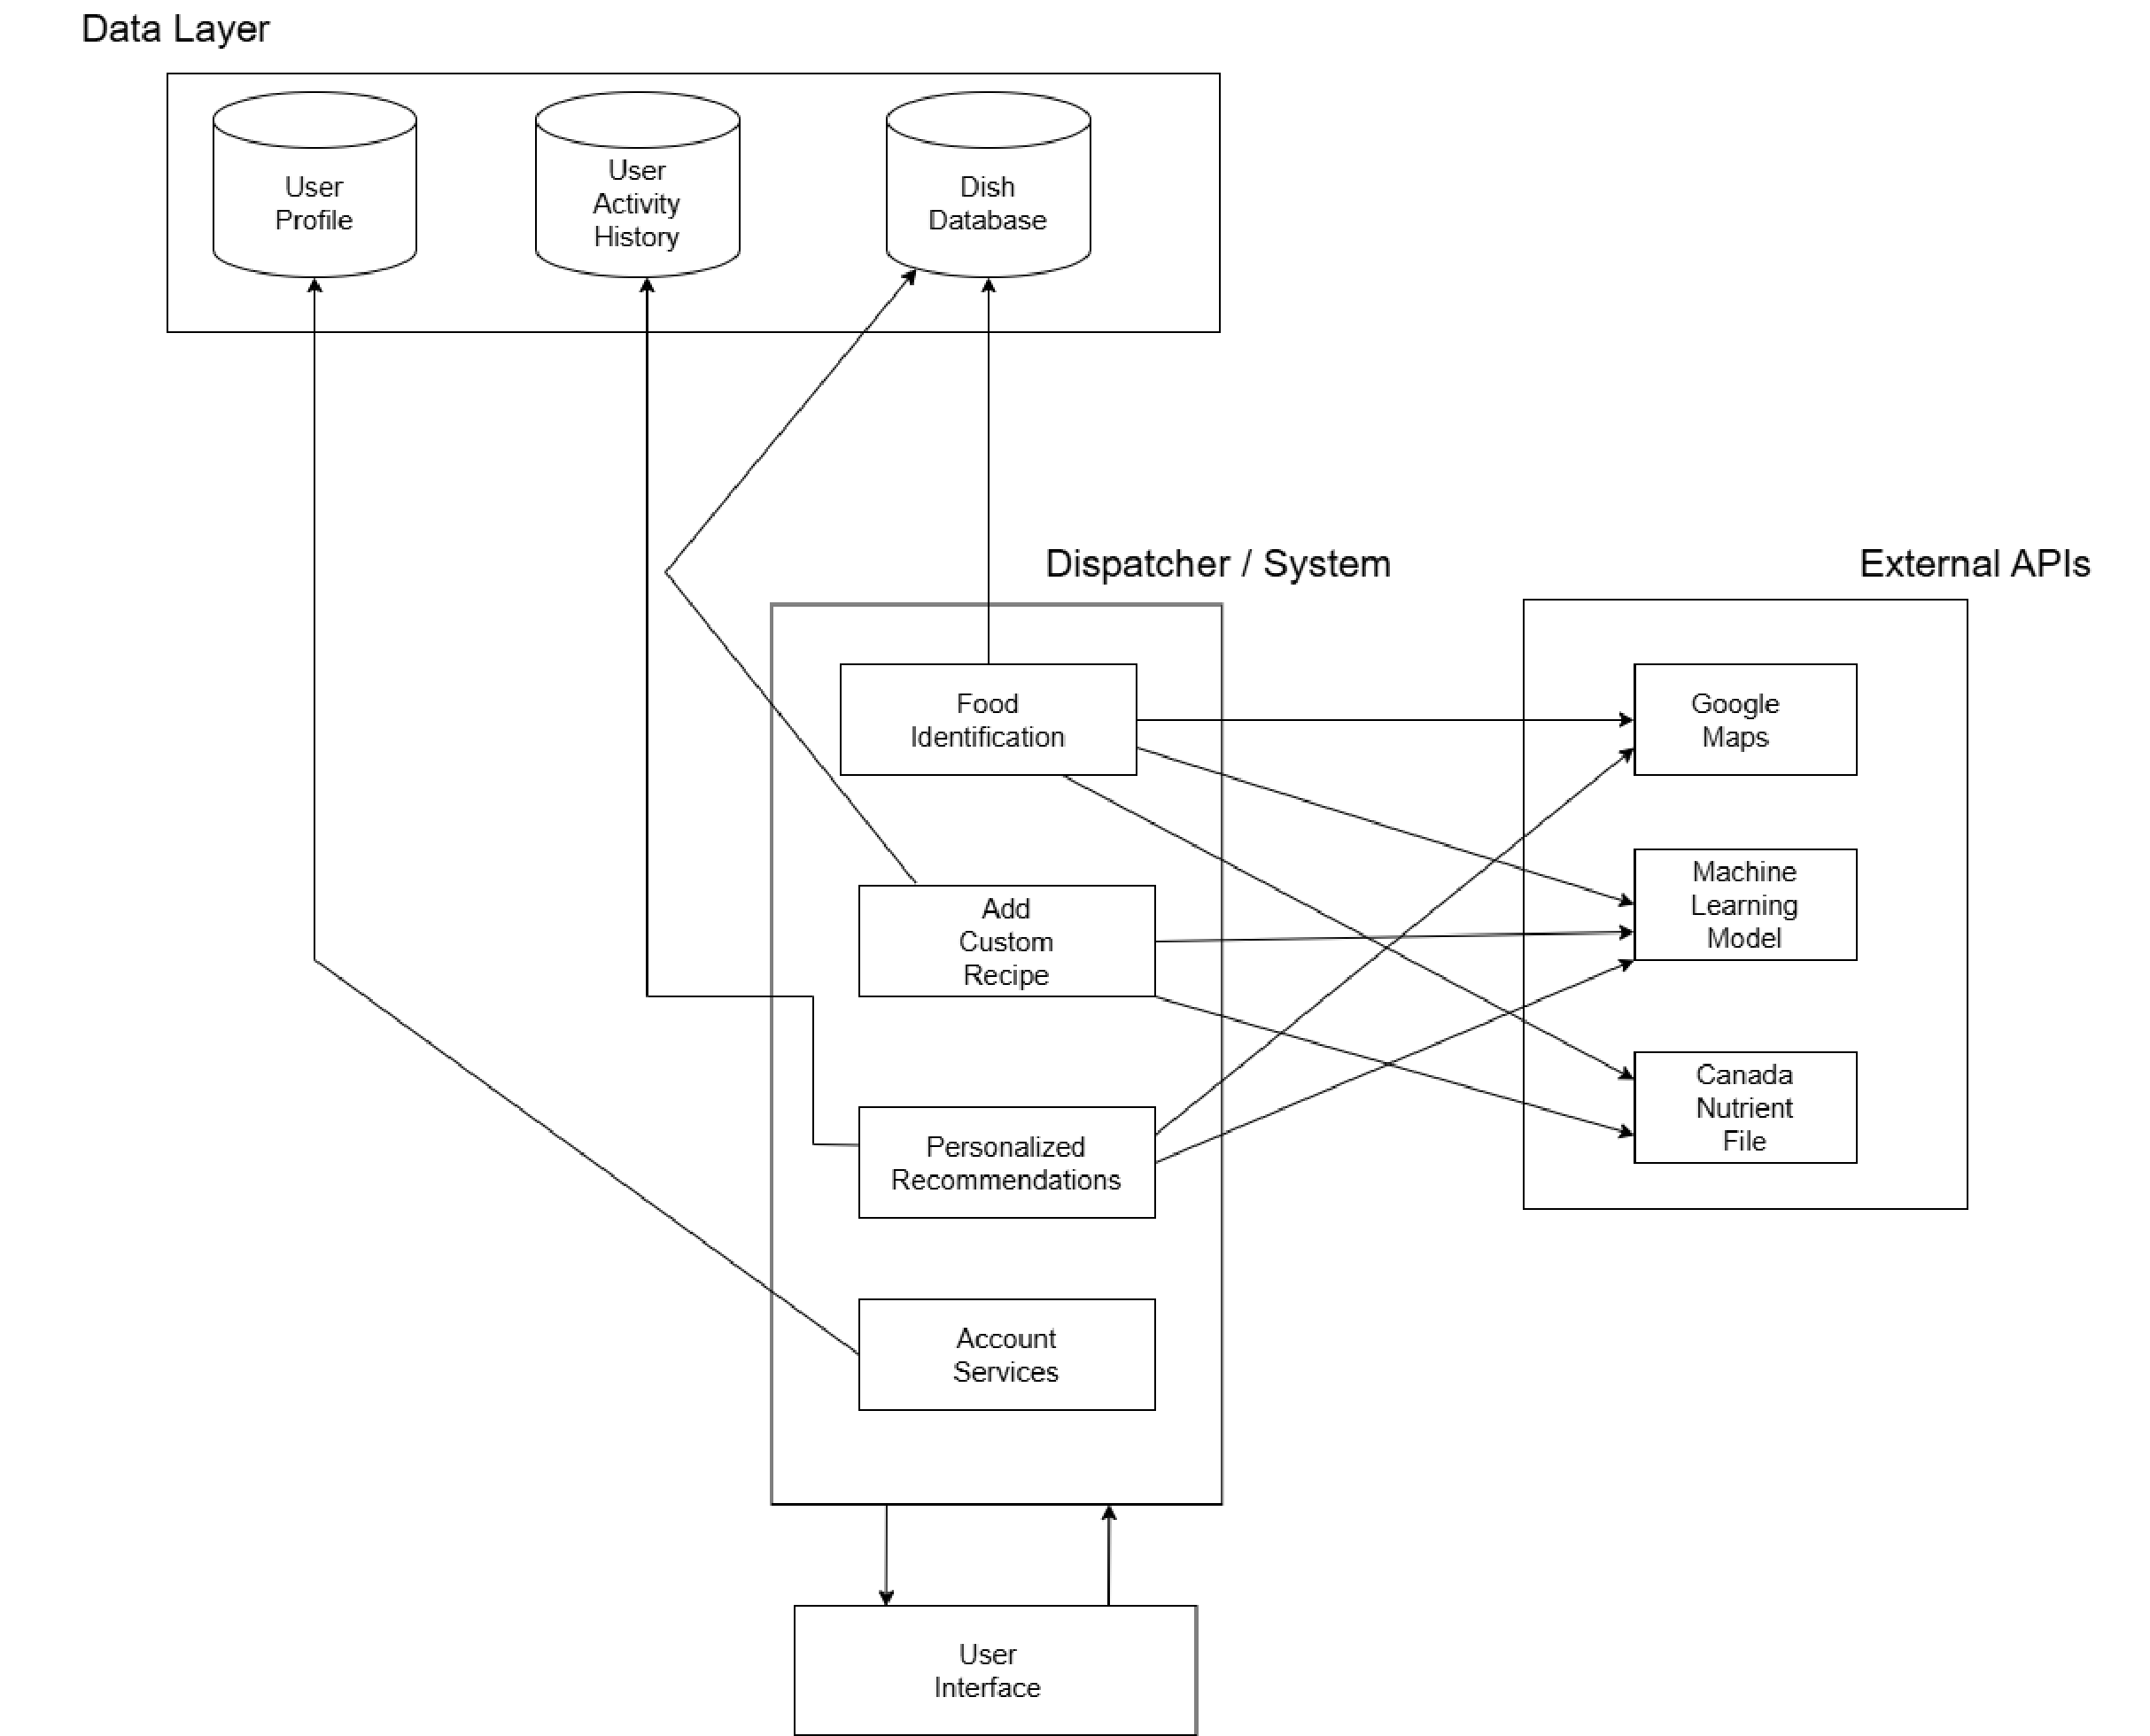
\includegraphics[width=\textwidth]{image/2.1_Diagram.pdf}
    \caption{\textbf{Figure 1:} System Diagram}
\end{figure}

\subsection{Product Functions}
\label{sub:product_functions}

The application's core features are divided into several modules. Each module contains functions that address the main needs of the user, such as creating an account or identifying unknown dishes.

\begin{table}[H]
\centering
\renewcommand{\arraystretch}{1.2} % Adjust row spacing
\begin{tabular}{|p{4cm}|p{10cm}|}
\hline
\textbf{Module} & \textbf{Functions} \\
\hline
\textbf{Account Management} &
\begin{itemize}
    \item \textbf{Create Account} – Allows new users to register within the app
    \item \textbf{Login} – Authenticates returning users for personalized features
    \item \textbf{Deactivate Account} – Removes or deactivates user data upon request
\end{itemize} \\
\hline
\textbf{Dish Inquiry} &
\begin{itemize}
    \item \textbf{Inquire About Unknown Food} – User provides an image, description, or ingredients for identification
    \item \textbf{Confirm or Reject Results} – User feedback helps refine AI accuracy
    \item \textbf{Handle Expert Conflicts} – Resolves differing predictions among the three experts
\end{itemize} \\
\hline
\textbf{Food Info \& Recipes} &
\begin{itemize}
    \item \textbf{Search Food Information} – Displays cultural background, recipe ideas, and dietary notes
    \item \textbf{Add Custom Recipe} – Allows users to submit personal recipes for future reference
    \item \textbf{Register Restaurant} – Enables addition of official dish details from restaurants
\end{itemize} \\
\hline
\textbf{Recommendation Engine} &
\begin{itemize}
    \item \textbf{Ask for Food Recommendations} – Suggests dishes based on user preferences
    \item \textbf{Refine Recommendations} – Improves suggestions using user feedback on accuracy
\end{itemize} \\
\hline
\textbf{Data Management} &
\begin{itemize}
    \item \textbf{Store User Interactions} – Logs confirmed/rejected identifications for AI training
    \item \textbf{Manage API Keys} – Secures AI service credentials within the codebase
    \item \textbf{Maintain Expert Models} – Coordinates updates among the three expert modules
\end{itemize} \\
\hline
\end{tabular}
\caption{Modules and Major Functions of the Dish-Identification App}
\label{tab:dish-functions}
\end{table}

\subsection{User Characteristics}
\label{sub:user_characteristics}

The target users for this dish-identification app are smartphone owners who enjoy discovering or learning more about various foods. Below is a general outline of their likely educational level, experience, and technical expertise:

\begin{enumerate}
    \item \textbf{Education Level:}
    \begin{itemize}
        \item \textbf{Basic to Moderate General Education}: Most users will have at least basic literacy, as they need to read short instructions and interpret on-screen results.
        \item \textbf{Above-Average Food Interest}: Given the nature of the app, users are likely more curious about cuisine than the average person. They may already recognize a variety of dishes or want to expand their knowledge of international foods and recipes.
    \end{itemize}
    
    \item \textbf{Experience:}
    \begin{itemize}
        \item \textbf{Familiar with Smartphone Apps}: Users typically have some background in using social media or taking screenshots of images. Since they capture food photos or screenshots, they already demonstrate comfort with basic smartphone functions.
        \item \textbf{No Special Experience Required}: The app is designed to be straightforward, so even someone using a food-discovery tool for the first time should be able to navigate features without difficulty (e.g., uploading an image, viewing results, and providing feedback).
    \end{itemize}
    
    \item \textbf{Technical Expertise:}
    \begin{itemize}
        \item \textbf{Basic App Navigation Skills}: The target user should know how to tap, swipe, or browse their camera roll. This covers a standard range of smartphone interactions.
        \item \textbf{Minimal Learning Curve}: The user interface is kept simple, with clear instructions and intuitive steps for uploading images or entering dish descriptions. Even older or less tech-savvy individuals can easily figure out how to identify a dish.
    \end{itemize}
\end{enumerate}

Overall, we expect a single user type or “persona” who is interested in identifying dishes and exploring information about them. Advanced technical or culinary knowledge is not a requirement, although a curiosity about world cuisines is common among most users of this application.
% End SubSection

\subsection{Constraints}
\label{sub:constraints}
% Begin SubSection
\begin{enumerate}
	\item \textbf{Data and Storage Constraints: }Data submitted by the user must be stored locally or in a cloud database, following Android data storage best practices. Storage limitations must be considered when handling high-resolution images to prevent excessive memory usage. If a cloud-based solution is used, the system must comply with API rate limits and data quotas.
	\item \textbf{Budget Constraints: }The project has a limited budget, which impacts the choice of third-party APIs, storage solutions, and computational resources. This means that free or open-source image recognition and NLP models should be prioritized to minimize costs.
	\item \textbf{Timeline Constraints: }The system must be developed within the allocated course duration, limiting the scope of certain advanced features such as restaurant API integration pr expanded multilingual support may need to be postponed to future versions.
	\item \textbf{Food Constraints: } They system will only work with and process foods and recipes that are edible by humans.
\end{enumerate}
% End SubSection

\subsection{Assumptions and Dependencies}
\label{sub:assumptions_and_dependencies}
% Begin SubSection
Assumptions made in interpreting what the software being developed is aiming to achieve:
	\begin{enumerate}
		\item The user will provide clear and distinguishable images of food items to enable accurate identification by the Image Recognition Expert.
		\item The Text Description Expert assumes that users will provide detailed descriptions of food items, including key attributes such as color, texture, taste, smell, or preparation method.
		\item The Ingredient-Based Expert assumes that users will provide a complete and accurate ingredient list for identification to work correctly.
		\item Users will have an active internet connection when interacting with the system for real-time processing and recommendations.
		\item The personalized recommendation system assumes that users submit multiple food items over time to generate tailored suggestions.
		\item The application assumes that it will operate on Android devices with a minimum required processing power and storage space to handle food image recognition and database queries.
	\end{enumerate}

Any other assumptions made that, if it fails to hold, could require you to change the requirements:
	%\item List each of the factors that affect the requirements stated in the SRS
	%\item These factors are not design constraints on the software but are, rather, any changes to them that can affect the requirements in the SRS
	\begin{enumerate}
		\item The system shall support the latest version of the Android operating system.
		\item Assume that the cost, availability, and accessibility of third-party APIs will remain unchanged.
		\item The system complies with the latest version of GDPR, PIPEDA, and other data protection regulations.
		\item The food database used for identification is accurate, regularly updated, and includes a diverse range of cuisines.
	\end{enumerate}

% End SubSection

\subsection{Apportioning of Requirements}
\label{sub:apportioning_of_requirements}
% Begin SubSection
\begin{enumerate}
    \item \textbf{Multilingual Support:} The initial version of the system will support English only, with additional language options planned for future updates.
    \item \textbf{Offline Mode:} Future versions will introduce offline functionality with local storage or caching for limited food recognition.
    \item \textbf{Integration with Third-Party Applications:} The system will expand to integrate with food-related services, including restaurants, delivery platforms like UberEats, and meal planning applications.
    \item \textbf{Voice Input and Accessibility Enhancements:} Later iterations will incorporate voice recognition, assisted voice input, and screen reader compatibility for improved accessibility.
\end{enumerate}
% End SubSection

% End Section
\section{Use Case Diagram}
\label{sec:use_case_diagram}
% Begin Section

\begin{figure}[H]
    \centering
    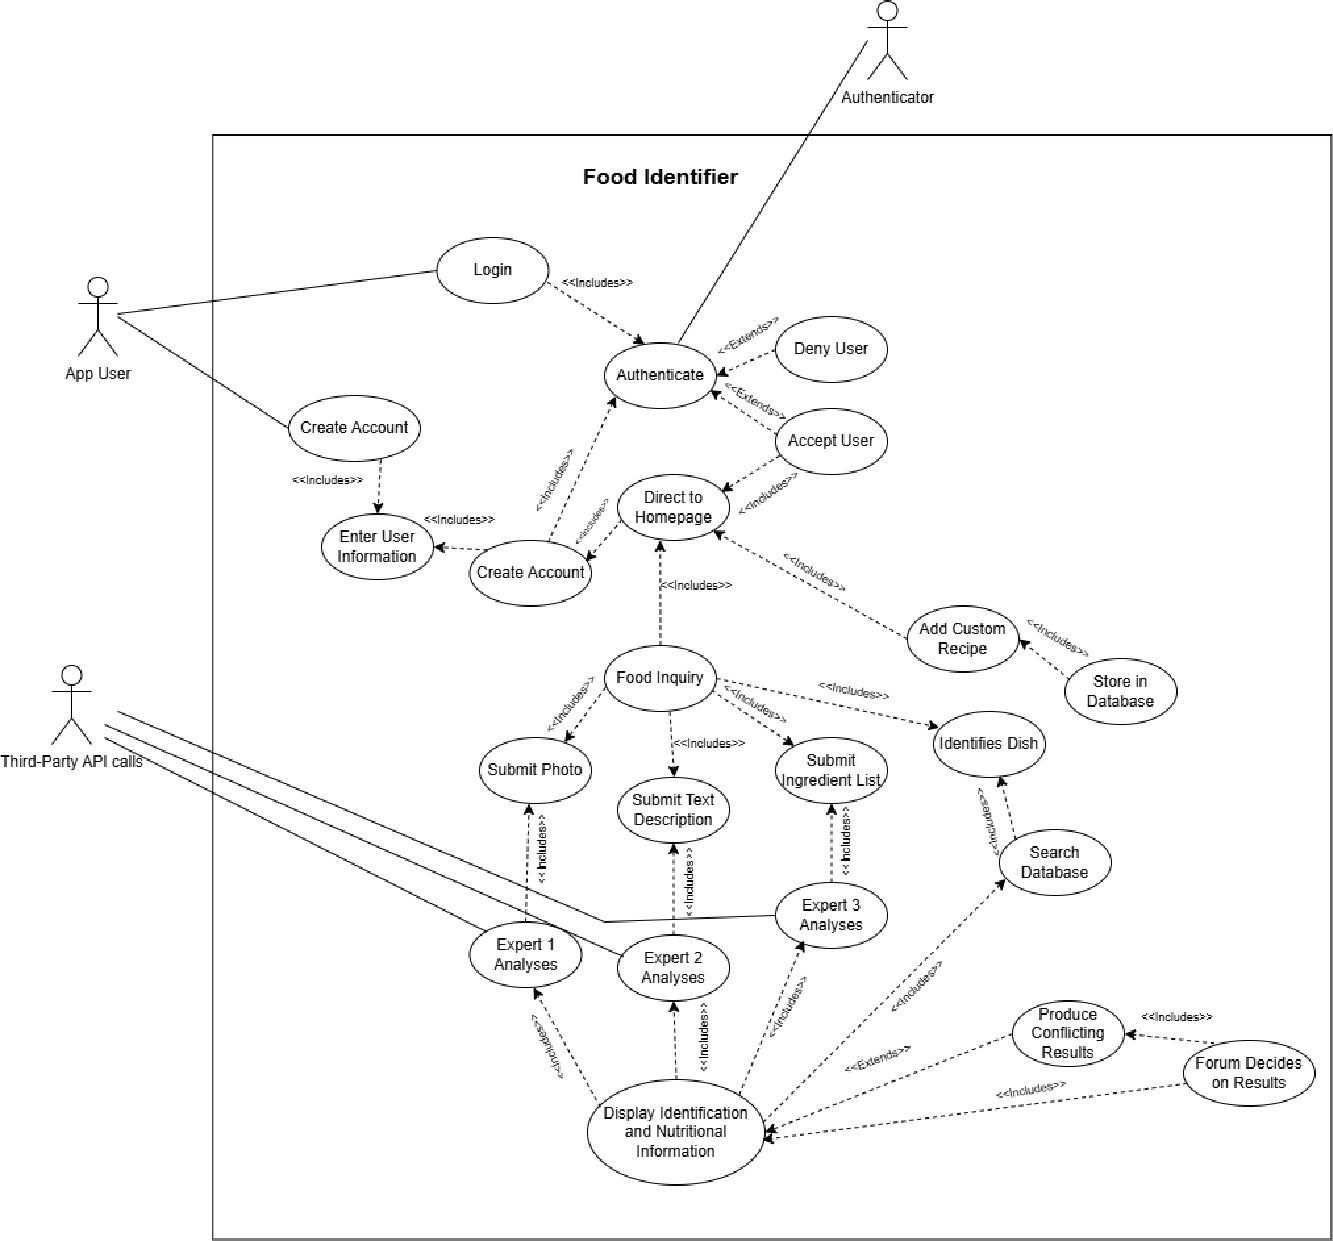
\includegraphics[width=\textwidth]{image/3_use_case_diagram.pdf}
    \caption{Use Case Diagram}
\end{figure}

%% End Section

\section{Highlights of Functional Requirements}
\label{sec:functional_requirements}
% Begin Section

\noindent {\bf Main Business Events:}
\begin{itemize}
	\item BE1 Inquiry of dish
	\item BE2 Create an account
	\item BE3 Login
	\item BE4 Add custom recipe
	\item BE5 Search food data
	\item BE6 Ask food recommendation
	\item BE7 Delete account
\end{itemize}

\noindent {\bf Viewpoints:}
\begin{itemize}
	\item VP1 User
	\item VP2 Health Canada
	\item VP3 Restaurant
	\item VP4 Security
	\item VP5 Customer Retention
\end{itemize}

\noindent {\bf Interpretation:} N/A \\

\begin{enumerate}[{\bf BE1.}]
	% Business Event 1.
	\item Inquiry of dish \#1
	
	\textbf{Pre-Condition:} User opens the application; they have an account and are logged in. The user also has some details of the dish to inquire about.
		% Viewpoints
		\begin{enumerate}[{\bf VP1.}]
			\item User \#1 \\
				\textbf{Main Success Scenario:} 
				\begin{enumerate}[{1.}]
					\item User presses a button to inquire about a dish.
					\item System prompts user to provide a photo of the food.
					\item User uploads a picture from their gallary or takes a photo of the food.
					\item System stores the picture.
					\item System prompts the user to provide textual description of the food.
					\item User types in description of food and presses a button to continue.
					\item System stores the textual description.
					\item System prompts user to provide the ingredients found on the dish.
					\item User enters the ingredient(s) found in the dish and presses a button to continue.
					\item System stores the ingredient list.
					\item System identifies the dish and displays the name of dish to the user as well as nutritional information.
				\end{enumerate}
				\textbf{Secondary Scenario:}
				\begin{enumerate}
					\item[4.i.] User does not provide a photo.
					\begin{enumerate}
						\item[4.i.1.] System does not store any picture.
					\end{enumerate}
					\item[4.ii.] User provides a blury picture.
					\begin{enumerate}
						\item[4.ii.1.] System warns user and ask user to try again.
					\end{enumerate}
				\end{enumerate}
				\begin{enumerate}
					\item[7.i.] User does not provide any textual description.
					\begin{enumerate}
						\item[7.i.1.] System stores an empty text.
					\end{enumerate}
				\end{enumerate}
				\begin{enumerate}
					\item[10.i.] User does not provide any ingredient.
					\begin{enumerate}
						\item[10.i.1.] System stores an empty ingredient list.
					\end{enumerate}
				\end{enumerate}
				\begin{enumerate}
					\item[11.i.] User did not provide either a picture, textual description, nor ingredient list
					\begin{enumerate}
						\item[11.i.1.] System does not accept inquiry request.
						\item[11.i.2.] System notifies user that no input data was given.
						\item[11.i.3.] System returns to home page.
					\end{enumerate}
					\item[11.ii.] System requests feedback of identified food.
					\begin{enumerate}
						\item[11.ii.1.] User enters feedback
						\item[11.ii.2.] System analyzes feedback and thanks user for feedback.
					\end{enumerate}
				\end{enumerate}

			\item Health Canada  \#2
				\begin{enumerate}
					\item[11.iii.] System must provide nutritional data in accordance with Health Canada's nutrition labelling policies \cite{CanadaNutrition}.
				\end{enumerate}
			\item Restaurant \#3
				\begin{enumerate}
					\item[11.iv.] System provides 4-5 star restaurants serving the returned dish.
				\end{enumerate}
			\item Security \#4 
				\begin{enumerate}
					\item[11.v.] System delete user provided photo from memory.
				\end{enumerate}
			\item Customer Retention \#5
				\begin{enumerate}
					\item[11.vi.] System saves identified dish in back-end data storage under user history.
				\end{enumerate}
		\end{enumerate}

		{\bf Global Scenario:} \\
		\textbf{Pre-Condition:} User opens the application; they have an account and are logged in. The user also has some details of the dish to inquire about. \\
		\textbf{Main Success Scenario:} 
		\begin{enumerate}[{1.}]
			\item User presses a button to inquire about a dish.
			\item System prompts user to provide a photo of the food.
			\item User uploads a picture from their gallary or takes a photo of the food.
			\item System stores the picture.
			\item System prompts the user to provide textual description of the food.
			\item User types in description of food and presses a button to continue.
			\item System stores the textual description.
			\item System prompts user to provide the ingredients found on the dish.
			\item User enters the ingredient(s) found in the dish and presses a button to continue.
			\item System stores the ingredient list.
			\item System identifies the dish and displays the name of dish to the user as well as nutritional information.
		\end{enumerate}
		\textbf{Secondary Scenario:}
		\begin{enumerate}
			\item[4.i.] User does not provide a photo.
			\begin{enumerate}
				\item[4.i.1.] System does not store any picture.
			\end{enumerate}
			\item[4.ii.] User provides a blury picture.
			\begin{enumerate}
				\item[4.ii.1.] System warns user and ask user to try again.
			\end{enumerate}
		\end{enumerate}
		\begin{enumerate}
			\item[7.i.] User does not provide any textual description.
			\begin{enumerate}
				\item[7.i.1.] System stores an empty text.
			\end{enumerate}
		\end{enumerate}
		\begin{enumerate}
			\item[10.i.] User does not provide any ingredient.
			\begin{enumerate}
				\item[10.i.1.] System stores an empty ingredient list.
			\end{enumerate}
		\end{enumerate}
		\begin{enumerate}
			\item[11.i.] User did not provide either a picture, textual description, nor ingredient list
			\begin{enumerate}
				\item[11.i.1.] System does not accept inquiry request.
				\item[11.i.2.] System notifies user that no input data was given.
				\item[11.i.3.] System returns to home page.
			\end{enumerate}
			\item[11.ii.] System requests feedback of identified food.
			\begin{enumerate}
				\item[11.ii.1.] User enters feedback
				\item[11.ii.2.] System analyzes feedback and thanks user for feedback.
			\end{enumerate}
			\item[11.iii.] System must provide nutritional data in accordance with Health Canada's nutrition labelling policies \cite{CanadaNutrition}.
			\item[11.iv.] System provides 4-5 star restaurants serving the returned dish.
			\item[11.v.] System delete user provided photo from memory.
			\item[11.vi.] System saves identified dish in back-end data storage under user history.
		\end{enumerate}

	% Business Event 2.
	\item Create an account \#2
	
	\textbf{Pre-Condition:} User has the mobile application downloaded on their android device and they do not have an account.
		% Viewpoints
		\begin{enumerate}[{\bf VP1.}]
			\item User \#1 \\
				\textbf{Main Success Scenario:} 
				\begin{enumerate}[{1.}]
					\item System prompts user to enter email address and password.
					\item User enters email and password for the application.
					\item System verifies user email has not been registed and emails a verification code.
					\item User enters emailed verification code on the application.
					\item System verifies verification code.
					\item System creates an account and stores in database.
					\item System prompts user to enter any allergies or dietary restrictions.
					\item User enters allergis or dietary restrictions or skips.
					\item Systems opens the application's home page.
				\end{enumerate}
				\textbf{Secondary Scenario:}
				\begin{enumerate}
					\item[2.i.] User does not provide a valid password.
					\begin{enumerate}
						\item[2.i.1.] System does not accept the password and reminds user of password criteria.
					\end{enumerate}
				\end{enumerate}
				\begin{enumerate}
					\item[4.i.] Entered verificaion code is not correct.
					\begin{enumerate}
						\item[4.i.1.] System does not accept code.
						\item[4.i.2.] Create account failed.
					\end{enumerate}
				\end{enumerate}

			\item Health Canada  \#2 \\
				N/A
			\item Restaurant \#3 \\
				N/A
			\item Security \#4 
			\begin{enumerate}
				\item[4.ii.] Verification time limit has passed.
				\begin{enumerate}
					\item[4.ii.1.] System does not accept code.
					\item[4.ii.2.] Create account failed.
				\end{enumerate}
			\end{enumerate}
			\item Customer Retention \#5 \\
				N/A
		\end{enumerate}

		{\bf Global Scenario:} \\
		\textbf{Pre-Condition:} User has the mobile application downloaded on their android device and they do not have an account. \\
		\textbf{Main Success Scenario:} 
		\begin{enumerate}[{1.}]
			\item System prompts user to enter email address and password.
			\item User enters email and password for the application.
			\item System verifies user email has not been registed and emails a verification code.
			\item User enters emailed verification code on the application.
			\item System verifies verification code.
			\item System creates an account and stores in database.
			\item System prompts user to enter any allergies or dietary restrictions.
			\item User enters allergis or dietary restrictions or skips.
			\item Systems opens the application's home page.
		\end{enumerate}
		\textbf{Secondary Scenario:}
		\begin{enumerate}
			\item[2.i.] User does not provide a valid password.
			\begin{enumerate}
				\item[2.i.1.] System does not accept the password and reminds user of password criteria.
			\end{enumerate}
		\end{enumerate}
		\begin{enumerate}
			\item[4.i.] Entered verificaion code is not correct.
			\begin{enumerate}
				\item[4.i.1.] System does not accept code.
				\item[4.i.2.] Create account failed.
			\end{enumerate}
			\item[4.ii.] Verification time limit has passed.
			\begin{enumerate}
				\item[4.ii.1.] System does not accept code.
				\item[4.ii.2.] Create account failed.
			\end{enumerate}
		\end{enumerate}

	% Business Event 3.
	\item Login \#3
	
	\textbf{Pre-Condition:} User opens the application and they have an account.
		% Viewpoints
		\begin{enumerate}[{\bf VP1.}]
			\item User \#1 \\
				\textbf{Main Success Scenario:} 
				\begin{enumerate}[{1.}]
					\item System prompts user to enter email and password.
					\item User enters login details.
					\item System authenticates login data.
					\item System brings user to home page.
				\end{enumerate}
				\textbf{Secondary Scenario:}
				\begin{enumerate}
					\item[2.i.] User forgets password.
					\begin{enumerate}
						\item[2.i.1.] User presses button to reset password.
						\item[2.i.2.] System sends password reset link to the email that the user provided if the email is registered.
					\end{enumerate}
				\end{enumerate}
			\item Health Canada  \#2 \\
				N/A
			\item Restaurant \#3 \\
				N/A
			\item Security \#4 
			\begin{enumerate}
				\item[3.i.] System authentication fails.
				\begin{enumerate}
					\item[3.i.1.] System warns user of invalid login.
					\item[3.i.2.] System permits retry of maximum 3 times before locking login feature for some time.
				\end{enumerate}
			\end{enumerate}
			\item Customer Retention \#5 \\
				N/A
		\end{enumerate}

		{\bf Global Scenario:} \\
		\textbf{Pre-Condition:} User opens the application and they have an account. \\
		\textbf{Main Success Scenario:} 
		\begin{enumerate}[{1.}]
			\item System prompts user to enter email and password.
			\item User enters login details.
			\item System authenticates login data.
			\item System brings user to home page.
		\end{enumerate}
		\textbf{Secondary Scenario:}
		\begin{enumerate}
			\item[2.i.] User forgets password.
			\begin{enumerate}
				\item[2.i.1.] User presses button to reset password.
				\item[2.i.2.] System sends password reset link to the email that the user provided if the email is registered.
			\end{enumerate}
			\item[3.i.] System authentication fails.
				\begin{enumerate}
					\item[3.i.1.] System warns user of invalid login.
					\item[3.i.2.] System permits retry of maximum 3 times before locking login feature for some time.
				\end{enumerate}
		\end{enumerate}

		% Business Event 4.
		\item Add custom recipe \#4
	
		\textbf{Pre-Condition:} User opens the application; they have an account and are logged in.
			% Viewpoints
			\begin{enumerate}[{\bf VP1.}]
				\item User \#1 \\
					\textbf{Main Success Scenario:} 
					\begin{enumerate}[{1.}]
						\item User presses button to add a recipe.
						\item \hypertarget{BE4.VP1.2} System prompts to enter name of recipe.
						\item User enters name of recipe.
						\item System prompts serving size info.
						\item User enters serving size info.
						\item System prompts to enter ingredient list.
						\item User enters ingredient list with their protion amount.
						\item System prompts user to write steps to making the dish.
						\item User provides the steps to make the dish.
						\item System saves the dish in database and notifies user of successful save.
					\end{enumerate}
					\textbf{Secondary Scenario:}
					\begin{enumerate}
						\item[6.i.] User types in ingredient that is not known to the system.
						\begin{enumerate}
							\item[6.i.1.] System notifies user that ingredient does not exist in the database.
							\item[6.i.2.] System does not add ingredient and ask user to provide a subsitute.
						\end{enumerate}
					\end{enumerate}
				\item Health Canada  \#2
					\begin{enumerate}
						\item[10.i.] Provided recipe is poisonous or hazardous.
						\begin{enumerate}
							\item[10.i.1.] System rejects recipe and does not add to the database.
							\item[10.i.2.] System provides information to user of why recipe is rejected.
						\end{enumerate}
					\end{enumerate}
				\item Restaurant \#3 \\
					N/A
				\item Security \#4 
					N/A
				\item Customer Retention \#5
					\begin{enumerate}
						\item[10.ii.] System should prompt an appreciation page for successful recipe that is added.
					\end{enumerate}
			\end{enumerate}
	
			{\bf Global Scenario:} \\
			\textbf{Pre-Condition:} User opens the application; they have an account and are logged in. \\
			\textbf{Main Success Scenario:} 
			\begin{enumerate}[{1.}]
				\item User presses button to add a recipe.
				\item \hypertarget{BE4.VP1.2} System prompts to enter name of recipe.
				\item User enters name of recipe.
				\item System prompts serving size info.
				\item User enters serving size info.
				\item System prompts to enter ingredient list.
				\item User enters ingredient list with their protion amount.
				\item System prompts user to write steps to making the dish.
				\item User provides the steps to make the dish.
				\item System saves the dish in database and notifies user of successful save.
			\end{enumerate}
			\textbf{Secondary Scenario:}
			\begin{enumerate}
				\item[6.i.] User types in ingredient that is not known to the system.
				\begin{enumerate}
					\item[6.i.1.] System notifies user that ingredient does not exist in the database.
					\item[6.i.2.] System does not add ingredient and ask user to provide a subsitute.
				\end{enumerate}
				\item[10.i.] Provided recipe is poisonous or hazardous.
					\begin{enumerate}
						\item[10.i.1.] System rejects recipe and does not add to the database.
						\item[10.i.2.] System provides information to user of why recipe is rejected.
					\end{enumerate}
				\item[10.ii.] System should prompt an appreciation page for successful recipe that is added.
			\end{enumerate}

		% Business Event 5.
		\item Ask for food recommendation \#5

		\textbf{Pre-Condition:} User opens the application; they have an account and are logged in.
			% Viewpoints
			\begin{enumerate}[{\bf VP1.}]
				\item User \#1 \\
					\textbf{Main Success Scenario:} 
					\begin{enumerate}[{1.}]
						\item User presses button for system to recommend food.
						\item System analyzes user data from user's database to recommend food and stores result in user history.
						\item \hypertarget{BE5.VP.1.3} System displays the recommened food with pictures and text.
					\end{enumerate}
					\textbf{Secondary Scenario:}
					\begin{enumerate}
						\item[2.i.] System does not have any user data..
						\begin{enumerate}
							\item[2.i.1.] System asks user for a cuisine category.
							\item[2.i.2.] System randomly picks a food from the selected cuisine category.
							\item[2.i.3.] System stores randomly chosen food in user history. 
						\end{enumerate}
					\end{enumerate}
				\item Health Canada  \#2
					\begin{enumerate}
						\item [2.ii.] System recommends food that respects the user's allergies and dietary restrictions.
					\end{enumerate}
				\item Restaurant \#3
					\begin{enumerate}
						\item[4.ii.] User presses button to get restaurant recommendation.
						\begin{enumerate}
							\item[4.ii.1.] System asks user to enter a postal code to serach in.
							\item[4.ii.2.] User enters postal code.
							\item[4.ii.3.] System provides top restaurants within the provided location.
						\end{enumerate}
					\end{enumerate}
				\item Security \#4 \\
					N/A
				\item Customer Retention \#5
					\begin{enumerate}
						\item[3.iii.] User likes the recommendation.
						\begin{enumerate}
							\item[3.iii.1.] System saves the recommended food in back-end data storage under user favorites.
							\item[3.iii.2.] System provides similar recommendations.
						\end{enumerate}
					\end{enumerate}
			\end{enumerate}
	
			{\bf Global Scenario:} \\
			\textbf{Pre-Condition:} User opens the application; they have an account and are logged in. \\
			\textbf{Main Success Scenario:} 
			\begin{enumerate}[{1.}]
				\item User presses button for system to recommend food.
				\item System analyzes user data from user's database to recommend food and stores result in user history.
				\item \hypertarget{BE5.VP.1.3} System displays the recommened food with pictures and text.
			\end{enumerate}
			\textbf{Secondary Scenario:}
			\begin{enumerate}
				\item[2.i.] System does not have any user data..
				\begin{enumerate}
					\item[2.i.1.] System asks user for a cuisine category.
					\item[2.i.2.] System randomly picks a food from the selected cuisine category.
					\item[2.i.3.] System stores randomly chosen food in user history. 
				\end{enumerate}
				\item[2.ii.] System recommends food that respects the user's allergies and dietary restrictions.
				\item[3.iii.] User likes the recommendation.
					\begin{enumerate}
						\item[3.iii.1.] System saves the recommended food in back-end data storage under user favorites.
						\item[3.iii.2.] System provides similar recommendations.
					\end{enumerate}
				\item[4.ii.] User presses button to get restaurant recommendation.
					\begin{enumerate}
						\item[4.ii.1.] System asks user to enter a postal code to serach in.
						\item[4.ii.2.] User enters postal code.
						\item[4.ii.3.] System provides top restaurants within the provided location.
					\end{enumerate}
			\end{enumerate}

	% Business Event 6.
	\item Search food data \#6
	
	\textbf{Pre-Condition:} User opens the application; they have an account and are logged in.
		% Viewpoints
		\begin{enumerate}[{\bf VP1.}]
			\item User \#1 \\
				\textbf{Main Success Scenario:} 
				\begin{enumerate}[{1.}]
					\item User presses button to search a food.
					\item System provides a text box and prompts user to enter the food name.
					\item User types the food names and presses enter.
					\item System searches in database and returns nutritional information of the food and a recipe.
				\end{enumerate}
				\textbf{Secondary Scenario:}
				\begin{enumerate}
					\item[2.i.] User types in food that is not known to the system.
					\begin{enumerate}
						\item[2.i.1.] System notifies user that food does not exist in the database.
						\item[2.i.2.] System suggests user to add a custom recipe of the food they search, return to \hyperlink{BE4.VP1.2}{BE4.VP1.2}.
					\end{enumerate}
				\end{enumerate}
			\item Health Canada  \#2
				\begin{enumerate}
					\item[4.i.] System must provide nutritional data in accordance with Health Canada's nutrition labelling policies \cite{CanadaNutrition}.
				\end{enumerate}
			\item Restaurant \#3
				\begin{enumerate}
					\item[4.ii.] User presses button to get restaurant recommendation.
					\begin{enumerate}
						\item[4.ii.1.] System asks user to enter a postal code to serach in.
						\item[4.ii.2.] User enters postal code.
						\item[4.ii.3.] System provides top restaurants within the provided location.
					\end{enumerate}
					
				\end{enumerate}
			\item Security \#4 
				N/A
			\item Customer Retention \#5
				\begin{enumerate}
					\item[3.iii.] User likes the food information page.
					\begin{enumerate}
						\item[3.iii.1.] System saves the searched food in back-end data storage under user favorites.
						\item[3.iii.2.] System provides some recommendations, return to \hyperlink{BE5.VP.1.3}{BE5.VP.1.3}.
					\end{enumerate}
				\end{enumerate}
		\end{enumerate}

		{\bf Global Scenario:} \\
		\textbf{Pre-Condition:} User opens the application; they have an account and are logged in. \\
		\textbf{Main Success Scenario:} 
		\begin{enumerate}[{1.}]
			\item User presses button to search a food.
			\item System provides a text box and prompts user to enter the food name.
			\item User types the food names and presses enter.
			\item System searches in database and returns nutritional information of the food and a recipe.
		\end{enumerate}
		\textbf{Secondary Scenario:}
		\begin{enumerate}
			\item[2.i.] User types in food that is not known to the system.
			\begin{enumerate}
				\item[2.i.1.] System notifies user that food does not exist in the database.
				\item[2.i.2.] System suggests user to add a custom recipe of the food they search, return to \hyperlink{BE4.VP1.2}{BE4.VP1.2}.
			\end{enumerate}
			\item[3.iii.] User likes the food information page.
				\begin{enumerate}
					\item[3.iii.1.] System saves the searched food in back-end data storage under user favorites.
					\item[3.iii.2.] System provides some recommendations, return to \hyperlink{BE5.VP.1.3}{BE5.VP.1.3}.
				\end{enumerate}
			\item[4.i.] System must provide nutritional data in accordance with Health Canada's nutrition labelling policies \cite{CanadaNutrition}.
			\item[4.ii.] User presses button to get restaurant recommendation.
				\begin{enumerate}
					\item[4.ii.1.] System asks user to enter a postal code to serach in.
					\item[4.ii.2.] User enters postal code.
					\item[4.ii.3.] System provides top restaurants within the provided location.
				\end{enumerate}
		\end{enumerate}

	% Business Event 7.
	\item Delete account \#7
	
	\textbf{Pre-Condition:} User opens the application; they have an account and are logged in.
		% Viewpoints
		\begin{enumerate}[{\bf VP1.}]
			\item User \#1 \\
				\textbf{Main Success Scenario:} 
				\begin{enumerate}[{1.}]
					\item User presses button for system to delete account.
					\item System warns user that they are deleting their account.
					\item User confirms to delete the account.
					\item System prompts reason of deleting the account.
					\item User enters reason of deleting.
					\item System saves reason of deleting to data storage.
					\item System removes user account from data storage.
					\item System notifies user account is deleted and returns to create account page.
				\end{enumerate}
				\textbf{Secondary Scenario:}
				\begin{enumerate}
					\item[3.i.] User cancels deletion
					\begin{enumerate}
						\item[3.i.1.] System returns to home page. 
					\end{enumerate}
				\end{enumerate}
				\begin{enumerate}
					\item[5.i.] User cancels deletion
					\begin{enumerate}
						\item[5.i.1.] System returns to home page. 
					\end{enumerate}
					\item [5.ii] User skips providing reason of deletion.
					\begin{enumerate}
						\item[5.ii.1.] System does not store any data about reason of deletion.
					\end{enumerate}
				\end{enumerate}
			\item Health Canada  \#2 \\
				N/A
			\item Restaurant \#3 \\
				N/A
			\item Security \#4 
				\begin{enumerate}
					\item [6.i.] System shall save the reason of deleting account without associating the user to it.
					\item [7.i.] System shall not have any user data in any of its data storage systems.
				\end{enumerate}
			\item Customer Retention \#5
				\begin{enumerate}
					\item[4.i.] System shall put the user's favourite food on the feedback form.
				\end{enumerate}
		\end{enumerate}

		{\bf Global Scenario:} \\
		\textbf{Pre-Condition:} User opens the application; they have an account and are logged in. \\
		\textbf{Main Success Scenario:} 
		\begin{enumerate}[{1.}]
			\item User presses button for system to delete account.
			\item System warns user that they are deleting their account.
			\item User confirms to delete the account.
			\item System prompts reason of deleting the account.
			\item User enters reason of deleting.
			\item System saves reason of deleting to data storage.
			\item System removes user account from data storage.
			\item System notifies user account is deleted and returns to create account page.
		\end{enumerate}
		\textbf{Secondary Scenario:}
		\begin{enumerate}
			\item[3.i.] User cancels deletion
			\begin{enumerate}
				\item[3.i.1.] System returns to home page. 
			\end{enumerate}
		\end{enumerate}
		\begin{enumerate}
			\item[4.i.] System shall put the user's favourite food on the feedback form.
			\item[5.i.] User cancels deletion
			\begin{enumerate}
				\item[5.i.1.] System returns to home page. 
			\end{enumerate}
			\item [5.ii] User skips providing reason of deletion.
			\begin{enumerate}
				\item[5.ii.1.] System does not store any data about reason of deletion.
			\end{enumerate}
			\item [6.i.] System shall save the reason of deleting account without associating the user to it.
			\item [7.i.] System shall not have any user data in any of its data storage systems.
		\end{enumerate}
		
\end{enumerate}

%End Section

\section{Non-Functional Requirements}
\label{sec:non-functional_requirements}

% Begin Section
\subsection{Look and Feel Requirements}
\label{sub:look_and_feel_requirements}
% Begin SubSection

\subsubsection{Appearance Requirements}
\label{ssub:appearance_requirements}
% Begin SubSubSection
\begin{enumerate}[{LF-A}1. ]
    \item \textit{The application shall use a visually appealing color scheme.} \\ \textbf{Rationale:} A visually unappealing color scheme will drive users away from the application.
    \item \textit{The application shall have a high contrast between all text and background elements so users can easily read the text.} \\
    \textbf{Rationale:} If the text is not easily readable, users will be discouraged from using the application
    \item \textit{No special prompt shall be required to display photos in application pages.} \\ \textbf{Rationale:} Requesting photos will make the usage more cumbersome, especially when browsing images of other food items in the library.
	\item \textit{The application shall mimic the layout, font and colour scheme of widely-used food ordering applications} \\ \textbf{Rationale:} Widely-used food ordering applications have conducted psychological studies to determine the best layout, font, and color 
\end{enumerate}
% End SubSubSection

\subsubsection{Style Requirements}
\label{ssub:style_requirements}
% Begin SubSubSection
\begin{enumerate}[{LF-S}1. ]
    \item \textit{The application shall use sans-serif for all its text.} \\ \textbf{Rationale:} Studies indicate it is more readable than serif counterparts \cite{Adobe}.
    \item \textit{The application shall use the same font for the same text category.} \\ \textbf{Rationale:} Unexplained variances in font will make the user experience needlessly more complex, which will discourage usage of the application.
    \item \textit{All text in the application shall conform to standard writing practices, including capitalization, spelling, grammar, bold text, italics, and underlining.} \\ \textbf{Rationale:} Deviating from standard writing convention will make the text needlessly harder to understand, which will discourage usage of the application.
\end{enumerate}
% End SubSubSection

% End SubSection

\subsection{Usability and Humanity Requirements}
\label{sub:usability_and_humanity_requirements}
% Begin SubSection

\subsubsection{Ease of Use Requirements}
\label{ssub:ease_of_use_requirements}
% Begin SubSubSection
\begin{enumerate}[{UH-EOU}1. ]
    \item \textit{The application shall have an intuitive user interface (UI) such that a user will easily grasp how to use the application.} \\ \textbf{Rationale:} If a user struggles to use the application, they will most likely not use it.
    \item \textit{The user experience (UX) shall be pleasant, especially for common use cases (e.g. taking or uploading pictures of a food item, inputting data for a food item, recieving the classification for a food item).}  \\ \textbf{Rationale:} If the user interface is not pleasant, it will incentivize users not to return to the application, and vice versa. Common use cases are emphasized because they occur far more often than their rare counterparts.
\end{enumerate}
% End SubSubSection

\subsubsection{Personalization and Internationalization Requirements}
\label{ssub:personalization_and_internationalization_requirements}
% Begin SubSubSection
\begin{enumerate}[{UH-PI}1. ]
    \item \textit{The application shall be available both in light mode and dark mode.} \\ \textbf{Rationale:} Some end users prefer light mode and some prefer dark mode, and having both modes will capture the full gamut \cite{NNgroup}. 
    \item \textit{Users shall be able to create accounts and have their public activity on the application tied to their account.} \\ \textbf{Rationale:} The benefits (cross-device support, sunk cost and user data collection), outweight the costs users are very familar with (increased friction and overhead) \cite{phiture2017}.
\end{enumerate}
% End SubSubSection

\subsubsection{Learning Requirements}
\label{ssub:learning_requirements}
% Begin SubSubSection
\begin{enumerate}[{UH-L}1. ]
	\item N/A
\end{enumerate}
% End SubSubSection

\subsubsection{Understandability and Politeness Requirements}
\label{ssub:understandability_and_politeness_requirements}
% Begin SubSubSection
\begin{enumerate}[{UH-UP}1. ]
	\item \textit{Responses shall be easily understood by the end user, including users with an advanced but not fluent understanding of English.} \\ \textbf{Rationale:} This application will be initially available only in English. Many people have an advanced but not fluent understanding of English \cite{USCensus} and simplifying the language will accommodate them without reducing the application's quality.
        \item \textit{Prompts should use polite phrases such as "please" when requesting and "thank you" after a user fulfills a request.} \\ \textbf{Rationale:} People appreciate polite language \cite{Standford}.
\end{enumerate}
% End SubSubSection

\subsubsection{Accessibility Requirements}
\label{ssub:accessibility_requirements}
% Begin SubSubSection
\begin{enumerate}[{UH-A}1. ]
	\item \textit{The application shall have a large text mode, where the size of the text is 18 points or greater.} \\\textbf{Rationale:} This will accommodate users with severe nearsightedness. The size of 18 pt is per the Web Content Accessibility Guidelines \cite{W3}
    \item \textit{The application shall be compatible with screen readers.} \\ \textbf{Rationale}: This will accommodate blind users who cannot see the application's visual content.
\end{enumerate}
% End SubSubSection

% End SubSection.

\subsection{Performance Requirements}
\label{sub:performance_requirements}
% Begin SubSection

\subsubsection{Speed and Latency Requirements}
\label{ssub:speed_and_latency_requirements}
% Begin SubSubSection
\begin{enumerate}[{PR-SL}1. ]
	\item The latency between sending a request for classification and getting the response, assuming a stable internet connection shall be no greater than three (3) seconds. \\ \textbf{Rationale:} Image processing standards demand a response within three (3) seconds \cite{Umentis}.
    \item \textit{The application's loading time shall not exceed two (2) seconds}. \\ \textbf{Rationale:} Roughly half of users will abandon an application that takes three (3) or more seconds.\cite{StoryLy}
    \item \textit{The latency between changing windows within an application shall be negligible, assuming a stable internet connection.} \\ \textbf{Rationale:} Users will readily abandon an application that takes a significant amount of time to load an application page.
\end{enumerate}
% End SubSubSection

\subsubsection{Safety-Critical Requirements}
\label{ssub:safety_critical_requirements}
% Begin SubSubSection
\begin{enumerate}[{PR-SC}1. ]
	\item \textit{The application shall reject attempts to classify non-food items as food} \\ \textbf{Rationale:} Naive users may believe the non-food classified as food is edible and eat it, which will lead to adverse effects.
    \item \textit{The system shall include allergen information, or warn users to ensure they are not allergic or intolerant to a food before trying it.} \\ \textbf{Rationale:} Users that eat food they are allergic or intolerant to may suffer adverse effects.
\end{enumerate}
% End SubSubSection

\subsubsection{Precision or Accuracy Requirements}
\label{ssub:precision_or_accuracy_requirements}
% Begin SubSubSection
\begin{enumerate}[{PR-PA}1. ]
	\item \textit{Virtually all information given in the application shall be verifiable by subject matter experts or generally reliable sources. The threshold for "virtually all" shall be no lesser than 99\% } \\ \textbf{Rationale:} Incorrect information will mislead users, which may lead to devastating consequences and users may stop using the application after discovering it duped them.
\end{enumerate}
% End SubSubSection

\subsubsection{Reliability and Availability Requirements}
\label{ssub:reliability_and_availability_requirements}
% Begin SubSubSection
\begin{enumerate}[{PR-RA}1. ]
	\item \textit{The application shall be available 99\% of the time.} \\ \textbf{Rationale:} This is a standard for a non-critical application, like this one \cite{ConcreteCMS}.
    \item \textit{The application shall inform users of any failure encountered, along with easily understandable advice to succeed on the next attempt. Usually, the advice would be to restart the application.} \\ \textbf{Rationale:} Users get frustrated when the application fails and should be given easy, reliable instructions to how to succeed on their next try to prevent disillusionment.
\end{enumerate}
% End SubSubSection

\subsubsection{Robustness or Fault-Tolerance Requirements}
\label{ssub:robustness_or_fault_tolerance_requirements}
% Begin SubSubSection
\begin{enumerate}[{PR-RFT}1. ]
	\item \textit{The application shall correct minor input and output errors when the intended meaning is obvious.} \\ \textbf{Rationale:} Humans and artificial intelligence make mistakes, and correcting minor errors will provide a smoother experience.
\end{enumerate}
% End SubSubSection

\subsubsection{Capacity Requirements}
\label{ssub:capacity_requirements}
% Begin SubSubSection
\begin{enumerate}[{PR-C}1. ]
	\item \textit{No human experts shall be required to compliment the non-human experts when a user uploads a picture of a food item, potentially with data about it to achieve a response.} \\ \textbf{Rationale:} This is part of the specification.
	\item \textit{The application shall be scalable to handle up to five million (5,000,000) concurrent users.} \\ \textbf{Rationale:} This is an upper bound for a growing mobile application, which may become very popular rapidly and would thus would have to scale rapidly \cite{Zeba}.
\end{enumerate}
% End SubSubSection

\subsubsection{Scalability or Extensibility Requirements}
\label{ssub:scalability_or_extensibility_requirements}
% Begin SubSubSection
\begin{enumerate}[{PR-SE}1. ]
    \item \textit{The application shall be able to handle ten (10) classification requests per second without any added latency.} \\ \textbf{Rationale:} This is a reasonable upper bound for a non-critical system, like this one.
\end{enumerate}
% End SubSubSection

\subsubsection{Longevity Requirements}
\label{ssub:longevity_requirements}
% Begin SubSubSection
\begin{enumerate}[{PR-L}1. ]
	\item \textit{The application shall last at least two years without any major updates, besides adding new functionality not in the initial release.} \\ \textbf{Rationale:} Software engineering principles should be utilized to make this extensive labor profitable.
\end{enumerate}
% End SubSubSection

% End SubSection

\subsection{Operational and Environmental Requirements}
\label{sub:operational_and_environmental_requirements}
% Begin SubSection

\subsubsection{Expected Physical Environment}
\label{ssub:expected_physical_environment}
% Begin SubSubSection
\begin{enumerate}[{OE-EPE}1. ]
	\item \textit{This application shall be compatible with all internal databases and artificial intelligence used by the system's non-human experts.} \\ \textbf{Rationale:} If the application is incompatible with the non-human experts, it will not work.
\end{enumerate}
% End SubSubSection

\subsubsection{Requirements for Interfacing with Adjacent Systems}
\label{ssub:requirements_for_interfacing_with_adjacent_systems}
% Begin SubSubSection
\begin{enumerate}[{OE-IA}1. ]
	\item \textit{This application shall be compatible with mobile devices running the Android platform.} \\ \textbf{Rationale:} This is part of the specification.
    \item \textit{This application shall conform to the terms of service of the Android Application store.} \\ \textbf{Rationale:} Sideloading may be dangerous and will discourage users from downloading the application \cite{Trio}. The only way for Android users to download it without sideloading is to be approved by the Android Application Store.
    \item \textit{If a parallel iOS mobile application is developed, it shall conform to the terms of service of the Apple Application store.} \\ \textbf{Rationale:} Sideloading may be dangerous and will discourage users from downloading the application \cite{Trio}. The only way for Apple users to download it without sideloading is to be approved by the Apple Application Store.
    
\end{enumerate}
% End SubSubSection

\subsubsection{Productization Requirements}
\label{ssub:productization_requirements}
% Begin SubSubSection
\begin{enumerate}[{OE-P}1. ]
	\item Not applicable.
\end{enumerate}
% End SubSubSection

\subsubsection{Release Requirements}
\label{ssub:release_requirements}
% Begin SubSubSection
\begin{enumerate}[{OE-R}1. ]
	\item \textit{This application shall be released for Android devices by April 8, 2025.} \\ \textbf{Rationale:} This is the release deadline given by the specification.
\end{enumerate}
% End SubSubSection

% End SubSection

\subsection{Maintainability and Support Requirements}
\label{sub:maintainability_and_support_requirements}
% Begin SubSection

\subsubsection{Maintenance Requirements}
\label{ssub:maintenance_requirements}
% Begin SubSubSection
\begin{enumerate}[{MS-M}1. ]
	\item \textit{The system shall be designed for easy debugging and troubleshooting, with clear logs and error reports.}
	\\ \textbf{Rationale:} Developers must be able to efficiently identify and resolve issues within the system. Clear logs and error reports provide essential information for troubleshooting and fixing bugs, ensuring smooth system operation and reducing downtime. This helps maintain app stability and performance over time.
\end{enumerate}
% End SubSubSection

\subsubsection{Supportability Requirements}
\label{ssub:supportability_requirements}
% Begin SubSubSection
\begin{enumerate}[{MS-S}1. ]
	\item \textit{The application shall be compatible with at least the last three major versions of Android and iOS.}
	\\ \textbf{Rationale:} Users must be able to access the app on a range of devices, including those running recent but not necessarily the latest operating system versions. Ensuring compatibility with at least the last three major versions of Android and iOS allows more users to access the app without requiring immediate upgrades, improving accessibility and usability while maintaining app performance and security.
\end{enumerate}
% End SubSubSection

\subsubsection{Adaptability Requirements}
\label{ssub:adaptability_requirements}
% Begin SubSubSection
\begin{enumerate}[{MS-A}1. ]
	\item \textit{The system architecture shall support future expansion by allowing the addition of new expert modules without requiring significant refactoring.}
	\\ \textbf{Rationale:} The system must be designed to accommodate future growth and enhancements. Allowing new expert modules to be added without major structural changes ensures scalability, reduces development effort, and maintains system stability as new features are introduced. This will help extend the system’s lifecycle and adaptability to evolving requirements.
\end{enumerate}
% End SubSubSection

% End SubSection

\subsection{Security Requirements}
\label{sub:security_requirements}
% Begin SubSection

\subsubsection{Access Requirements}
\label{ssub:access_requirements}
% Begin SubSubSection
\begin{enumerate}[{SR-AC}1. ]
	\item \textit{User authentication shall be required for storing identification history, ensuring only authorized users access their data.}
	\\ \textbf{Rationale:} To protect user privacy and security, only authenticated users must be able to store and access their identification history. This prevents unauthorized access to sensitive information and ensures that personal data remains secure within the system.
\end{enumerate}
% End SubSubSection

\subsubsection{Integrity Requirements}
\label{ssub:integrity_requirements}
% Begin SubSubSection
\begin{enumerate}[{SR-INT}1. ]
    \item \textit{The app must inform and ask users for the usage of their information.}
    \\ \textbf{Rationale:} This is a requirement under the Google Play Developer Distribution Agreement \cite{GooglePlayAgreement}. Users must be explicitly informed about how their data will be used, ensuring transparency and compliance with privacy policies.

    \item \textit{The app must provide users a legally adequate privacy notice.}
    \\ \textbf{Rationale:} This is a requirement under the Google Play Developer Distribution Agreement \cite{GooglePlayAgreement}. A clear and legally adequate privacy notice ensures users understand their rights and how their personal data is managed, promoting trust and regulatory compliance.
\end{enumerate}
% End SubSubSection

\subsubsection{Privacy Requirements}
\label{ssub:privacy_requirements}
% Begin SubSubSection
\begin{enumerate}[{SR-P}1. ]
	\item \textit{The system shall allow users to delete their stored identification history on request.}
	\\ \textbf{Rationale:} Users must have control over their personal data. Allowing users to delete their stored identification history ensures compliance with privacy regulations and enhances user trust. This feature provides transparency and empowers users to manage their data as needed.
	\item \textit{The system shall permanently delete all user data when a user account is removed from the system.}
	\\ \textbf{Rationale:} Retaining user data after account deletion serves no functional purpose and poses potential privacy risks. To ensure compliance with data protection principles outlined in PIPEDA \cite{PIPEDA1}, the application shall enforce complete data removal upon account deletion.
\end{enumerate}
% End SubSubSection

\subsubsection{Audit Requirements}
\label{ssub:audit_requirements}
% Begin SubSubSection
\begin{enumerate}[{SR-AU}1. ]
	\item \textit{The system shall log all expert consultations and final decisions, including timestamps and user interactions, for auditing purposes.}
	\\ \textbf{Rationale:} Maintaining logs of expert consultations and decisions ensures accountability and traceability. These logs help track system usage, detect potential issues, and support compliance with regulatory or internal audit requirements.
\end{enumerate}
% End SubSubSection

\subsubsection{Immunity Requirements}
\label{ssub:immunity_requirements}
% Begin SubSubSection
\begin{enumerate}[{SR-IM}1. ]
	\item \textit{The system must not accept unexpected input.}
	\\ \textbf{Rationale:} The system must be protected against security vulnerabilities caused by invalid or malicious input. Preventing unexpected input helps mitigate risks such as SQL injection, cross-site scripting (XSS), and buffer overflow attacks, ensuring the system remains secure and reliable for users.
\end{enumerate}
% End SubSubSection

% End SubSection

\subsection{Cultural and Political Requirements}
\label{sub:cultural_and_political_requirements}
% Begin SubSection

\subsubsection{Cultural Requirements}
\label{ssub:cultural_requirements}
% Begin SubSubSection
\begin{enumerate}[{CP-C}1. ]
	\item \textit{The application shall ensure that identifications are culturally sensitive and do not promote stereotypes or biases.}
	\\ \textbf{Rationale:} Users must feel respected and represented fairly when using the application. Ensuring that identifications are culturally sensitive helps prevent discrimination, reduces potential harm, and promotes inclusivity. This approach fosters a positive user experience and aligns with ethical and legal standards for diversity and equity.
\end{enumerate}
% End SubSubSection

\subsubsection{Political Requirements}
\label{ssub:political_requirements}
% Begin SubSubSection
\begin{enumerate}[{CP-P}1. ]
	\item \textit{The application shall remain politically neutral and shall not classify or provide recommendations based on politically sensitive topics, ideologies, or national symbols.}
	\\ \textbf{Rationale:} The system must ensure fairness and avoid influencing users based on political views. Maintaining political neutrality prevents bias, reduces potential conflicts, and promotes inclusivity, allowing users to engage with the application without concerns about ideological influence or discrimination.
\end{enumerate}
% End SubSubSection

% End SubSection

\subsection{Legal Requirements}
\label{sub:legal_requirements}
% Begin SubSection

\subsubsection{Compliance Requirements}
\label{ssub:compliance_requirements}
% Begin SubSubSection
\begin{enumerate}[{LR-COMP}1. ]
	\item \textit{All personal information collected (including personal information given to third parties for processing purposes) must be protected.}
	\\ \textbf{Rationale:} Users must have confidence that their personal data is secure. Protecting collected information ensures compliance with privacy regulations, such as PIPEDA Fair Information Principle 1 - Accountability\cite{PIPEDA1}.
	\item \textit{The purposes for all personal information being collected (including personal information given to third parties for processing purposes) must be identified before or at the time it is being collected.}
    \\ \textbf{Rationale:} Users must be informed about why their personal information is being collected. Clearly identifying data collection purposes ensures transparency, builds user trust, and aligns with PIPEDA Fair Information Principle 2 - Identifying Purposes \cite{PIPEDA2}.  

    \item \textit{The knowledge and consent of the user for all personal information collected (including personal information given to third parties for processing purposes) is required.}
    \\ \textbf{Rationale:} Users must have control over their personal data. Obtaining their knowledge and consent before collecting information ensures informed decision-making and aligns with PIPEDA Fair Information Principle 3 - Consent \cite{PIPEDA3}.  

    \item \textit{Only the personal information that is needed to fulfill a legitimate identified purpose must be collected.}
    \\ \textbf{Rationale:} Collecting only necessary personal information reduces privacy risks and enhances user confidence in the system. This ensures compliance with data minimization principles and follows PIPEDA Fair Information Principle 4 - Limiting Collection \cite{PIPEDA4}.  

    \item \textit{All the personal information collected (including personal information given to third parties for processing purposes) may be used or disclosed only for identified purposes (purposes for which it was collected) except when user consents or under any legal obligation(s).}
    \\ \textbf{Rationale:} Users must have clarity on how their data is used. Restricting the use or disclosure of personal information to its identified purposes prevents misuse and aligns with PIPEDA Fair Information Principle 5 - Limiting Use, Disclosure, and Retention \cite{PIPEDA5}.  
\end{enumerate}
% End SubSubSection

\subsubsection{Standards Requirements}
\label{ssub:standards_requirements}
% Begin SubSubSection
\begin{enumerate}[{LR-STD}1. ]
    \item \textit{The application should not use notifications for promotional or advertisement purposes.}
    \\ \textbf{Rationale:} This is a standard for app quality in terms of the visual experience, as defined by Google's Core App Quality guidelines from Android Developers \cite{GoogleCoreAppQuality}. Notifications should be used appropriately to enhance user experience and should not be misused for cross-promotion or advertisements.

    \item \textit{Touch targets in the app should have a size of at least 48dp.}
    \\ \textbf{Rationale:} Ensuring that touch targets are at least 48dp improves accessibility and usability, as recommended by Google's Core App Quality guidelines from Android Developers \cite{GoogleCoreAppQuality}. This helps users interact more easily with UI elements and reduces frustration.

    \item \textit{Any personal or sensitive data should not be logged to the system log or a log specific to the app.}
    \\ \textbf{Rationale:} This is a standard for app quality in terms of privacy and security, as outlined in Google's Core App Quality guidelines from Android Developers \cite{GoogleCoreAppQuality}. Logging sensitive data can lead to security vulnerabilities and data exposure, which must be avoided.

    \item \textit{The application's internal storage should be used to store any sensitive data.}
    \\ \textbf{Rationale:} Storing sensitive data in internal storage enhances security and prevents unauthorized access, as per best practices defined in Google's Core App Quality guidelines from Android Developers \cite{GoogleCoreAppQuality}.
\end{enumerate}
% End SubSubSection

% End SubSection

% End Section

\section{Innovative Feature}

The chosen innovative feature is to inquire food items for which users seek classification by the region of its cusine, ingredients used to prepare it, and its style of preparation. 
This feature benefits users who are curious about the origins of specific dishes, want to explore new cuisines, and seek to expand their culinary experiences.
This innovative feature will keep user actively involved because it offers an engaging way to learn about diverse food cultures.
Other innovative features we came up with include:

\begin{itemize}
	\item Ability to add custom recipe to the system, allowing users to share their creation with others.
	\item Request food recommendations based on the user's previous searches.
	\item Considerations of user's allergies and dietary restrictions.
	\item A browsing format enabling users to see dishes previously classified by the application.
	\item A rating system, allowing users to recommend to others which dishes to try and which to avoid
	\item Partnerships with restaurants, with an emphasis on small, local restaurants, which will support the restaraunt industry
	through promoting their unique food offerings.
\end{itemize}

\appendix
\section{Division of Labour}
\label{sec:division_of_labour}
% Begin Section

\textbf{Imran Chowdhury:}
\begin{enumerate}
	\item Sections 2.1 -- 2.3; Product Perspective, Product Functions, and User Characteristics.
	\item Provided feedback for sections 5.1, 5.2, 5.3, and 5.4.
	\item Contributed to Section 1.2 and provided extensive feedback on its initial draft to ensure its alignment with the project mission.
\end{enumerate}

\textbf{Michael Roberts:}
\begin{enumerate}
	\item TODO
\end{enumerate}

\textbf{Sathurshan Arulmohan:}
\begin{enumerate}
	\item Section 4; Creating and writing out the Business Events and scenarios for each view point.
	\item Provided feedback to 1.2, 2.1, all of section 5 and 6.
	\item Updated Latex with references for 1.4 using IEEE format.
	\item Wrote out section 1.1.
\end{enumerate}

\textbf{Tanisha Tasnin:}
\begin{enumerate}
	\item TODO
\end{enumerate}

\textbf{Zifan Si:}
\begin{enumerate}
	\item TODO
\end{enumerate}

% End Section

\end{document}

%------------------------------------------------------------------------------
